\documentclass[12pt]{article}

\usepackage{tikz}
%\usepackage{russ}
\usepackage[left=2.5cm,right=2.5cm,top=2.5cm,bottom=2.5cm]{geometry}
%\usepackage[russian]{babel}
\usepackage{cmap}

\usepackage[T2A]{fontenc}
%\usepackage[cp1251]{inputenc}
\usepackage{amssymb, amsmath, amsthm}
\usepackage{epsfig,graphicx}
\bibliographystyle{harvard}

%\pagestyle{empty}
\pagenumbering{arabic}

%\voffset          -2.0cm \textwidth          11cm \textheight         16cm
%\topmargin           0mm \oddsidemargin       5mm \emergencystretch=3pt

%\setlength{\textwidth}{6in}

\newtheorem{theorem}{Theorem}[section]
\newtheorem{lemma}[theorem]{Lemma}
\newtheorem{proposition}[theorem]{Proposition}
\newtheorem{corollary}[theorem]{Corollary}

%\setlength{\parindent}{4em}
%\setlength{\parskip}{1em}
\renewcommand{\baselinestretch}{1.3}

%\baselineskip{1}
\everymath{\displaystyle}
%
\begin{document}

\title{On the feasibility for the system of quadratic equations
%\thanks{Grants or other notes
%about the article that should go on the front page should be
%placed here. General acknowledgments should be placed at the end of the article.}
}
%\subtitle{Do you have a subtitle?\\ If so, write it here}

%\titlerunning{Short form of title}        % if too long for running head

\author{Anatoly Dymarsky \&   Elena Gryazina  \& Boris Polyak%etc.
}

%\authorrunning{Short form of author list} % if too long for running head

%\institute{B. Polyak and E. Gryazina are with \at
% Institute of Control Sciences, 119779, 65 Profsoyuznaya Street, Moscow, Russia \\
%    and \\
 %   Skoltech Center for Energy Systems, Skolkovo Institute of Science and Technology, 143026, Skolkovo Innovation Center, \\ 3 Nobel Street, Moscow, Russia \\
%    \email{gryazina@gmail.com}           %  \\
%             \emph{Present address:} of F. Author  %  if needed
%}


\maketitle

\begin{abstract} We consider several problems related to quadratic equations
that arise in power flow analysis, discrete optimization,
uncertainty analysis and physical applications. we provide deep
analysis for the image of the space of variables under quadratic map
(the feasibility domain). There are several classes of quadratic
maps representing the image convexity, while in general the image is
nonconvex, nevertheless, demonstrates hidden convexity structure.

We propose numerical procedure to check the feasibility for the
individual quadratic transformation. On this way we provide
sufficient condition for infeasibility and investigate the numerical
algorithms exploiting convex relaxation of quadratic mappings for
discovering nonconvexity. Identifying convex parts of the image we
verify feasibility of certain point. Finally, we address such
problems as membership oracle and boundary oracle for the quadratic
image as well as local convexity analysis.

AC power flow equations seem to be the natural application. $N-1$
contingency assessment, maximum loadability regime search as well as
other problem of power systems security and stability analysis can
be addressed via the proposed methodology.

{\bf Keywords} Quadratic Maps, \and Feasibility, \and Hidden
Convexity, \and Convex Relaxations, \and  Power Flow analysis
% \PACS{PACS code1 \and PACS code2 \and more}
% \subclass{MSC code1 \and MSC code2 \and more}
\end{abstract}

\section{Introduction}
\label{intro}

[EXPECTED...]

%%%%%%%%%%%%%%%%%%%%%%%%%%%%%%%%%%%%%%%%%%%%%%%%%%%%%%%%%%%%%%%%%%%%%%%%%%%%%%%
%
%  paper structure
%
%%%%%%%%%%%%%%%%%%%%%%%%%%%%%%%%%%%%%%%%%%%%%%%%%%%%%%%%%%%%%%%%%%%%%%%%%%%%%%%

The paper is organized as follows. In Section \ref{known_facts} we
formulate the problem, emphasize the role of convexity of the image
under quadratic transformations and refer to known results on
convexity for particular classes of quadratic functions. We
formulate the main results in Section \ref{certif}. It contains the
analysis of the image in terms of supporting hyperplane,
certificates of convexity/ nonconvexity. We also develop efficient
algorithms to obtain the certificates. The algorithms exploit convex
relaxation technique and so called ``boundary oracle'' for convex
domains. Section \ref{power_flow} is devoted for the application of
the proposed routine for the problem of checking attainability of
operation regimes.
%Power Flow equations do not fit directly to any
%of the known classes, thus our approach is different
%--- we try to check convexity/ nonconvexity of an individual
%quadratic map.
Section \ref{num_res} contains results on numerical simulation.
Conclusions and directions for the future work can be found in final
Section \ref{conclusion}.

%%%%%%%%%%%%%%%%%%%%%%%%%%%%%%%%%%%%%%%%%%%%%%%%%%%%%%%%%%%%%%%%%%%%%%%%%%%%%%%%%%%%
\section*{Notations}

 We consider
multidimensional quadratic mapping $f: \mathbb{R}^n \rightarrow
\mathbb{R}^m$ or $f: \mathbb{C}^n \rightarrow \mathbb{R}^m$ of the
form
\begin{align}
f(x) & = (f_1(x), f_2(x), \dots,f_m(x))^T \nonumber \\
 f_i(x) & = x^* A_i x + b_i^*x + x^* b_i , \quad i = 1,\dots, m \leq
 n. \label{ex:map}
\end{align}

and its image
$$
 F  =  \{f(x): x \in \mathbb{R}^n \text{~or~} x\in \mathbb{C}^n\}\subseteq\mathbb{R}^m,
$$
where $^*$ denotes transposition for real variable mapping or
hermitian conjugation for complex variable mapping. $F$ is the image
of the whole space under the mapping $f$, we call it also {\it
feasibility region}. Denote by $G = \text{conv}(F)$ its convex hull.

$\partial F_c$ --- the boundary points of $F$ touched by the
supporting hyperplane with normal vector $c \in \mathbb{R}^m$. We
use notation $C_{+}$ for the set of $c$ such that $A_c =
\sum\limits_{i=1}^m c_i A_i \succ 0$. For $c\in C_{+}$ it is clear
that $\partial F_{c}$ consists of a single point. Otherwise, we say
$c \in C_{-}$.

% $f(-(\sum c_i A_i)^{-1} \sum c_i b_i)$, $z_0 = \min\limits_{f\in
%F}(c, f)$

%{\bf Good directions:} $c_{+}$: $A_{c_{+}} \succ 0$


%{\bf Bad directions:} $c_{BAD}$ or $c_{NC}$ or ???

%Boundary points minimizing $(c_{NC}, f)$  (a sort of the
%intersection with the supporting hyperplane) are described as
%$$
%\varphi(\alpha) = f(\alpha e+d) = f^0 +f^1 \alpha +f^2\alpha^2,
%\quad d = -A_{c_{NC}}^{+}b_{c_{NC}}
%$$

For symmetric (hermitian) matrices $\langle X,Y\rangle$ =
trace$(XY)$, and $X\succeq 0$ denotes nonnegative definite matrix
$X$.

%%%%%%%%%%%%%%%%%%%%%%%%%%%%%%%%%%%%%%%%%%%%%%%%%%%%%%%%%%%%%%%%%%%%%%%%%%%%%%%
%
%  SECTION
%
%%%%%%%%%%%%%%%%%%%%%%%%%%%%%%%%%%%%%%%%%%%%%%%%%%%%%%%%%%%%%%%%%%%%%%%%%%%%%%%

\section{Problem formulation and the role of convexity}
\label{known_facts}

Quadratic transformations arise in discrete optimization,
uncertainty analysis, physical applications.  A variety of problems
from combinatorial and continuous mathematical programming can be
recast as quadratic minimization under quadratic constraints. These
are binary integer programs (linear programs with binary variables),
polynomial programs, scheduling problems of minimizing total length
of the schedule under certain precedence constraints and machine
availability constraints. Besides, a number of problems for power
flow analysis involves quadratic maps. In general all the problems
mentioned above are nonconvex, nevertheless, demonstrate hidden
convexity structure and admit extremely efficient convex
relaxations. The idea of convex relaxations for quadratic problems
goes back to \cite{Shor}; recent results and references can be found
in \cite{Zhang} and \cite{LuoIEEE}. Similar ideas and technique give
the convex hull for the image set $F$, see also \cite{Beck}.

We examine several problems regarding the image of quadratic map
$F$:
\begin{enumerate}
  \item Feasibility or Membership Oracle.

\centerline{For the given $y^0\in\mathbb{R}^m$ determine whether
$y^0 \in F$.}
  This problem is shown to be NP-hard \cite{Ramana_NPhard94} but it is extremely vital for numerous applications.
  \item Boundary Oracle.
\begin{center}For $y^0\in F$ and arbitrary direction $d$ find the maximal $t$

such that for all $\tau \in [0, t]$ $y^0 + \tau d \in F$.
\end{center}
Any iterative method for this problem requires the solution of the
feasibility problem in every step. In contrast, the boundary points
as well as their pre-images described by supporting hyperplane with
normal $c\in C_{+}$ can be easily calculated. Nevertheless, boundary
oracle is needed when the boundary point in a certain direction $d$
is of interest. Besides, boundary oracle procedure allows us to
implement Markov-Chain Monte Carlo techniques for efficient sampling
even in nonconvex domains.

  \item Convexity Oracle.

   \centerline{Check the convexity of $F$ for particular $f$.}
   In the general setting we do not assume that matrices $A_i$ are
sign-definite; nevertheless $F$ sometimes occur to be convex
(``hidden convexity'' property). For a few low-dimensional classes
of $f$ the image convexity is guaranteed:
\begin{itemize}
  \item $x\in \mathbb{R}^n$ or $x\in \mathbb{C}^n$, $m = 2$, $b_i \equiv 0$; \cite{Dines}, \cite{Brickman}.
  \item $x\in \mathbb{R}^n$, $m = 2$, $b_i \neq 0$ and $c_1 A_1 + c_2 A_2 \succ
  0$;   \cite{polyak98}. For $x\in \mathbb{C}^n$ see Lemma
  \ref{lem:m2compex} below.
  \item $x\in \mathbb{C}^n$, $m = 3$, $b_i \equiv 0$; \cite{HT}
  \item  $x\in \mathbb{R}^n$, $m = 3$ and there exists a positive-definite  linear combination of matrices
$A_1, A_2, A_3$ and $b_i\equiv 0$; see \cite{Calabi},
\cite{polyak98}.
\end{itemize}
Besides, if $b_i\equiv 0$ and matrices $A_i$ commute, then $F$ is
convex \cite{Fradkov}. In general, checking the convexity of $F$ for
particular $f$, $m>2$ is NP-hard.

  \item Convex subparts of $F$.

 If $A_i$ have positive off-diagonal entries, then ``positive
  part of $F$'' is convex (i.e. $F+R^m_{+}$ is convex) \cite{KK}. In
  the general case, instead of analyzing the whole image $F$ some local information can
 be useful. One approach for local analysis exploits the fact that
 the image of the small ball $\|x - x^0\|\leq \varepsilon$ remains
 convex for $\varepsilon \leq \varepsilon_{\max}$ \cite{polyak01}, \cite{Dymarsky_SmallBall}. But there is no
 regular routine for the tight estimation of $\varepsilon_{\max}$
 and we desire to describe convex subpart in $\mathbb{R}^m$ rather then in  the pre-image
 space.
\end{enumerate}

%%% interconnections
There are links between the problems mentioned above. The convexity
is the crucial property. Once the image of $f$ is recognized as
convex Membership and Boundary Oracles appear immediately. The
convex relaxation is tight and it allows us to implement powerful
numerical procedures of convex optimization (Linear Matrix
Inequalities, duality theory). Namely, we can answer if a particular
$y^0$ is feasible or not without solving equations and searching for
the pre-image $x^0: f(x^0) = y^0$. On the other hand, the
infeasibility of certain $y^0$ can be checked easily if $y^0 \not
\in G$. When the image $F$ is nonconvex but its part $F_c$ is known
to be convex we obtain {\it limited} Membership and Boundary Oracles
that provide feasibility and boundary points efficiently for $y \in
F_c$.


%%% we propose
To solve the bunch of problems described above we provide several
routines, their application for particular $f$ and $y^0$ is
schematically demonstrated in Fig. \ref{fig:scheme}.

%\begin{figure}[h]
%\centerline{\includegraphics[width=10cm]{Scheme01.eps}}
%\caption{Diagram for examining particular $f$ [TO
%PLOT!].}\label{fig:scheme}
%\end{figure}

%\begin{center}
%\begin{tikzpicture}[sibling distance=10em,
%  every node/.style = {shape=rectangle, rounded corners,
%    draw, align=center,
%    top color=white, bottom color=blue!20}]]
%  \node {$[f, y_0]$}
%        child { node {sufficient conditions Theorem 3.2 }
%      child { node {...}
%        %child { node {relation sign} }
%        %child { node {several places} }
%        %child { node {center} }
%        }
%      child { node {MO for
%$y_0$} } };
%\end{tikzpicture}
%\end{center}

The whole routine contains three main blocks.
\begin{enumerate}
  \item Sufficient condition for infeasibility that checks if given $y^0$ is in the
convex hull of $F$. Obviously, for convex images the sufficient
condition is also necessary.
  \item Nonconvexity certificate. Randomized numerical algorithm that
discovers nonconvexity with probability one. The output of the
algorithm is the set of vectors $C_{-}$ such that supporting
hyperplane with normal $c \in C_{-}$ touches the image $F$ in more
than one point and the subset of $C_{=}\subseteq C_{-}$
characterizing nonconvex boundary.
  \item Theory for cutting convex subpart of $F$. Indeed, for the boundary points
of $F$ where the supporting hyperplane with normal $c\in C_{+}$
touches the single point with pre-image $x^0$, the convexity is
preserved for the image of a small ball $\|x - x^0\|\leq
\varepsilon$. This in turn can be reformulated as the convexity of
the intersection of $F$ and $(c,f) \leq z_{\max}$. Equipped with the
set $C_{-}$ from nonconvexity certificate we efficiently calculate
the appropriate $z_{\max}$.
\end{enumerate}

For membership oracle one should start with the sufficient condition
for infeasibility for $y^0$. If $y^0$ is not infeasible the
convexity issue arises and nonconvexity certificate is applied. If
we obtain $C_{-} = \oslash$ it is the strong support of the
convexity assumption and efficient Membership and Boundary Oracles
are straightforward. When the procedure discovers nonempty $C_{-}$,
under certain conditions we are able to cut convex subpart $F_c$ by
the inequality $(c, f)\leq z_{\max}$. This provides limited
Membership and Boundary Oracle and we are able to check if $y^0$
belongs to this convex subpart. Finally, the proposed routine does
not solve all the completely. There still remain blind zones for
membership oracle since we can't certify feasibility for $y^0 \not
\in F_c$.

%There are some other classes of quadratic transformations with
%convex images, however typically $F$ is nonconvex; numerous examples
%will be provided later.


%%%%%%%%%%%%%%%%%%%%%%%%%%%%%%%%%%%%%%%%%%%%%%%%%%%%%%%%%%%%%%%%%%%%%%%%%%%%%%%
%
%  SECTION
%
%%%%%%%%%%%%%%%%%%%%%%%%%%%%%%%%%%%%%%%%%%%%%%%%%%%%%%%%%%%%%%%%%%%%%%%%%%%%%%%

\section{Feasibility certificates for convex and nonconvex images}
\label{certif}

In the general case we do not know in advance if the image of the
quadratic map is convex or not. We provide the computational routine
to address the problems from Section \ref{known_facts}. In this
section we describe all the steps above and formulate the final
algorithm.

\subsection{Sufficient condition for infeasibility}

We remind some known facts on convex hull for quadratic image and exploit it to
formulate the sufficient condition for infeasibility.

\begin{theorem}\emph{(Convex hull)}

The convex hull for the feasibility set $F$ is
$$
G = \text{conv}(F) = \{ \mathcal{H}(X): X\succeq 0, X_{n+1, n+1} =
1\},
$$
where $X = X^* \in \mathbb{C}^{(n+1)\times(n+1)}$, $\mathcal{H}(X) =
(\langle{H}_1,X\rangle, \langle{H}_2,X\rangle, \dots,
\langle{H}_m,X\rangle)^T$, $H_{i} = \left(\begin{array}{cc}
                                                  A_i & b_i \\
                                                  b_i^* & 0 \\
                                                \end{array}
                                              \right).
$
\end{theorem}
Hence we can provide simple sufficient conditions for checking if a
particular point $y^0\in \mathbb{R}^m$ is infeasible (does not belong to $F$).
Indeed, for $y^0 \in F$ it is necessary to have $y^0\in G$, that is to solve corresponding linear
matrix inequality (LMI):
\begin{equation}\label{eq:LMI1}
 \mathcal{H}(X) = y^0, \quad X\succeq 0, \quad X_{n+1, n+1} = 1.
\end{equation}

Alternatively, if the point does not belong to the convex domain it
can be separated by a certain hyperplane. We introduce the variable
$c\in \mathbb{R}^m$ and construct matrix $A_c = \sum c_i A_i$,
vector $b_c= \sum c_i b_i$ and block matrix
\begin{equation}\label{eq:Hc} H(c) = \left(
                                                \begin{array}{cc}
                                                  A_c & b_c \\
                                                  b_c^* & -(c,y^0) \\
                                                \end{array}
                                              \right).\end{equation}
Vector $c$ is the normal for separating hyperplane (Fig.
\ref{fig:sep_hyp}) and the sufficient condition for $y^0 \not\in F$
has the form:
\begin{figure}[htb]
\centerline{\includegraphics[width=12cm]{sep_hyperplane2.eps}}
\caption{Infeasibility certificate via separating
hyperplane.}\label{fig:sep_hyp}
\end{figure}

\begin{theorem}\emph{(Sufficient condition)}\label{th:suff_cond}

If for given $y^0$ there exists $c$ such that $H(c)\succ 0$
(\ref{eq:Hc}), then $y^0$ is infeasible.
\end{theorem}
\begin{proof}
Via Schur complement $H(c)\succ 0$ $\Leftrightarrow$ $A_c\succ 0$
and $-(c,y^0) - b_c^* A_c^{-1} b_c >0$. But the latter inequality
means
$$
(c,y^0) < - b_c^* A_c^{-1} b_c = \min x^* A_c x + 2x^* b_c =
\min\limits_{y\in G} (c,y).
$$
It means that there exists the separating hyperplane, defined by its
normal $c$ that strictly separates $y^0$ and $G= conv(F)$, hence
$y^0$ does not belong to $F$.
\end{proof}

\begin{corollary}\emph{(Convex case)}

If the image $F$ is convex the sufficient condition given by Theorem
\ref{th:suff_cond} is also necessary.
\end{corollary}

Holding $H(c)\preceq 0$ for all $c$ implies feasibility of $y^0$
just for convex $F$. Therefore we examine convexity of $F$.

\subsection{Nonconvexity certificate}

We examine convexity/nonconvexity of $F$ in terms of the
intersection with the supporting hyperplane with normal vector $c$.
The geometry of $\partial F_c$ is different depending on the
spectrum of $A =\sum c_i A_i$. First, if $A$ is sign-definite the
corresponding supporting hyperplane intersects $F$ at the unique
point $\partial F_c$. Further we denote these $c$ as $c_{+}$.
Second, if $A$ has both positive and negative eigenvalues then there
is no corresponding supporting hyperplane in this case because $F$
stretches to infinity in both directions along $c$. Finally, when
$A$ is semi-definite and singular we discover nonconvexity checking
a few extra conditions.

\begin{theorem}\emph{(Nonconvexity certificate)}\label{th:noconv_cert}

Let $m \geq 3$, $n \geq 3$, $b_i \neq 0$, and for some $c = (c_1,
c_2, \dots, c_m)^T\neq 0$, the matrix $A = \sum c_i A_i \succeq 0$
has a simple zero eigenvalue $A e = 0$, and for $b = \sum c_i b_i$
we have $b^*e + e^*b = 0$. Let also exist $e^0$: $A x^0 = -b$.
Denote $x^{\alpha} = \alpha e+e^0$, $f^{\alpha} = f(x^{\alpha}) =
f^0 +f^1 \alpha +f^2\alpha^2$. If $f^1 \not \parallel f^2$
%$|(f^1, f^2)| < \|f^1\|\cdot \|f^2\|$,
then $F$ is nonconvex.
\end{theorem}

Geometrically the condition implies that the linear function $(c,f)$
attains its minimum on $F$ at points $f^{\alpha}$ only. But parabola
$f^{\alpha}$ is nonconvex, thus the supporting hyperplane touches
$F$ on a nonconvex set. Further we denote by $C_{-}$ vectors
satisfying the condition of Theorem \ref{th:noconv_cert}.

Now the main problem is to find $C_{-}$ (if exists) and hence
discovers nonconvexity of the feasible set. At the first glance,
sampling in $c$ can be applied. Take $c\in \mathbb{R}^m$ and
minimize $(c,f)$ on $G$ if such minimum exists. If $A_c = \sum c_i
A_i\succ 0$ the minimum is unique and obtained at rank-1 matrix
$xx^*$, $x = -A_c^{-1}b_c$, $b_c=\sum c_ib_i$, and $x$ gives a
pre-image for the boundary point of $F$. However, to identify
nonconvexity we should find $c$ such that $A$ is singular. The
probability of this event is zero if we sample $c$ randomly.

\begin{figure}[h]
\centerline{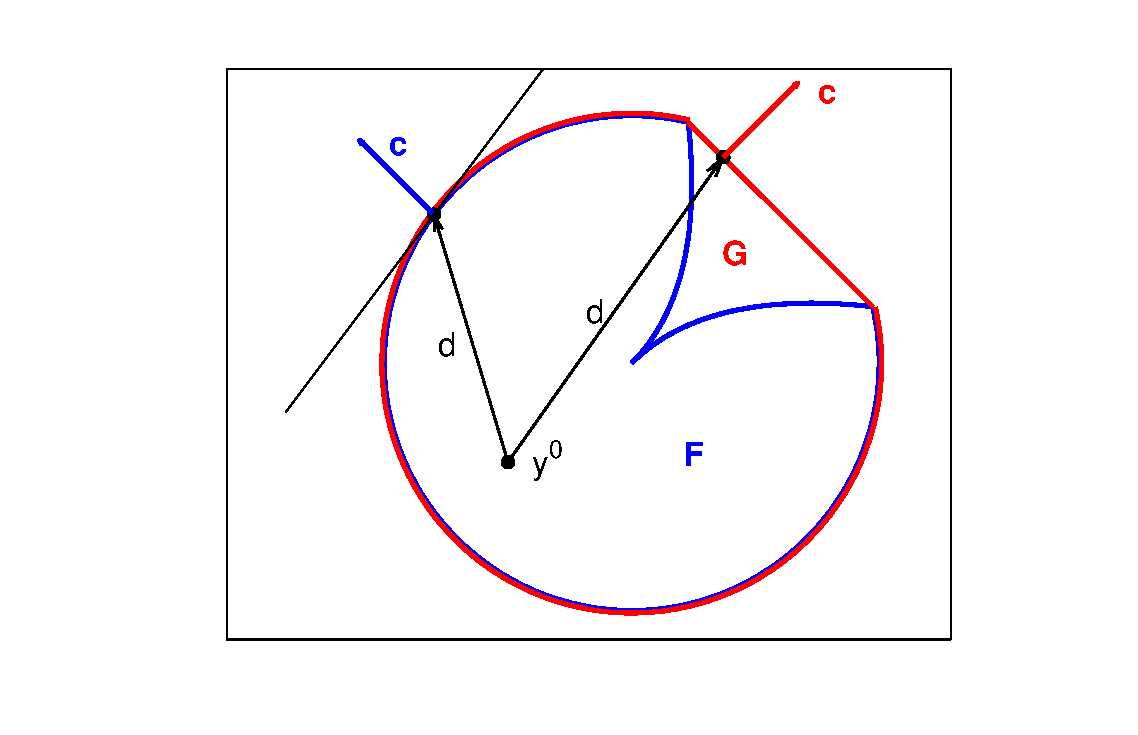
\includegraphics[width=12cm]{alg_idea20.eps}}
\caption{Idea of the nonconvexity
certificate.}\label{fig:nonconv_idea}
\end{figure}

For efficient search of vectors $C_{-}$  satisfying the condition of
Theorem \ref{th:noconv_cert} we construct so called \emph{boundary
oracle} for $G$ and exploit its dual problem. The idea of the
nonconvexity certificate is demonstrated in Fig.
\ref{fig:nonconv_idea}. Boundary oracle is the procedure that
returns the boundary point for given $y^0 \in G$ and the arbitrary
direction $d \in \mathbb{R}^m$. For a convex hull of $F$ the
following Semidefinite Program (SDP) \cite{Boyd} with variables
$t\in \mathbb{R}$, $X = X^* \in \mathbb{R}^{(n+1)\times(n+1)}$
specifies the boundary point $y^0 + td$ of the convex hull:
\begin{align}
\max & ~t  \label{BO_SPD}\\
\mathcal{H}(X) & = y^0 + td \nonumber \\
X & \succeq 0 \nonumber\\
X_{n+1, n+1} & = 1. \nonumber
\end{align}


If we obtain rank$(X) = 1$ for the solution of (\ref{BO_SPD}) we
claim that the obtained boundary point is on the boundary of $F$.
Otherwise, the boundary point of the convex hull does not belong to
$F$ and lies on the ''flat part'' of the boundary of $G$.

On the other hand the dual problem to (\ref{BO_SPD}) gives us normal
vector $c$ for the boundary point:
\begin{align}
\min & ~\gamma + (c, y^0)  \label{dual_BO}\\
(c,d)& = -1 \nonumber \\
%X & \succeq 0 \nonumber\\
H & = \left(
        \begin{array}{cc}
          \sum c_i A_i & \sum c_i b_i \\
          \sum c_i b_i^* & \gamma \\
        \end{array}
      \right) \succeq 0
 \nonumber
\end{align}
This is again SDP in variables $c$ and $\gamma$.

Equipped with boundary oracle technique (which provides both a
boundary point of $G$ and the normal vector $c$ in this point) we
are able to discover vectors $c$ to identify nonconvexity as in
Theorem \ref{th:noconv_cert}. In our approach we sample random
directions $d$ (instead of $c$) and the probability of finding a
boundary point on a ``flat part'' of the boundary of $G$ (which
correspond to nonconvex $F$) is positive.

\begin{theorem}\emph{(Efficiency of the nonconvexity certificate)}\label{th:prob1}

Let $d\in U(S^{m-1})$ be uniformly distributed on the unit sphere
and the random variable
$$
\varphi(d) = \left\{\begin{array}{l}
                      1, \quad \text{ if the solution } $c$ \text{ of the problem (\ref{dual_BO}) satisfies Theorem \ref{th:noconv_cert}}\\
                      0, \quad \text{ otherwise.}
                    \end{array}
 \right.
$$
Then if the image $F$ is nonconvex the expectation
$\mathbb{E}(\varphi)>0$.
\end{theorem}

To conclude it is the strong support of the convexity assumption if
we do not discover nonconvexity after checking large number of
directions $d$ for various $y^0\in G$.

\subsection{Certifying convex parts of the image}

Discovering nonconvexity in terms of $C_{-}$ does not help directly
to check feasibility for the given $y^0$. Nevertheless, exploiting
local convexity \cite{Dymarsky_cuttingArX} of $F$ gives us
opportunity to cut convex part of the image.

Consider $c_{+}$ such that $A_{+} = \sum (c_{+})_i A_i \succ 0$ the
supporting hyperplane orthogonal to $c_{+}$ touches $F$ in a single
point $\partial F_{c_{+}}$ with pre-image $x^0 = -A_{+}^{-1}b_{+}$,
$b_{+} = \sum (c_{+})_i b_i$. The image of the ellipsoid centered in
$x^0$
$$
(x - x^0)^*A_{+}(x - x^0) \leq \varepsilon^2
$$ preserves convexity for $\varepsilon \leq
\varepsilon_{\max}$. Moreover, every ellipsoid $(x - x^0)^*A_{+}(x -
x^0) \leq \varepsilon^2$ is mapped into its own hyperplane
$(c_{+},f) = (c_{+}, f(x^0)) + \varepsilon^2$ and we can certify
convexity of
\begin{equation}
\label{eq:conv_cut} F\cap\{(c_{+}, f) \leq   z_{\max}\}, \quad
z_{\max} = (c_{+}, f(x^0)) + \varepsilon_{\max}^2.
\end{equation}

We call the inequality in (\ref{eq:conv_cut}) {\it convex cut} and
illustrate it in Fig. \ref{fig:cut}.
\begin{figure}[htb]
\centerline{\includegraphics[width=16cm]{cut.eps}} \caption{Cutting
convex part.}\label{fig:cut}
\end{figure}
% [FRENCH BAGUETTE IS PREFERABLE]

There are several estimates for $\varepsilon_{\max}$ (and
$z_{\max}$) requiring various computational effort. But the
knowledge of $C_{-}$ -- the set of vectors $c$ such that supporting
hyperplane orthogonal to $c$ touches the image $F$ in ''flat edge''
and discovers nonconvexity -- brings the clue to find $z_{\max}$
exactly.

Indeed, the nonconvex boundary points lie at the parabola $f(\alpha
e + e^0)$ and nearest point to $\partial F_{c_{+}}$ can be found
straightforward as $z_c = \min\limits_{\alpha} (c_{+}, f(\alpha e +
e^0))$. Finally, $z_{\max}$ is obtained minimizing $z_c$ among all
discovered nonconvexities
\begin{equation}
\label{eq:z_max} z_{\max} = \min\limits_{c\in C_{-}} z_c.
\end{equation}


\subsection{Numerical algorithm}

Now we summarize all the reasoning above in the algorithmic form.

\paragraph{Algorithm}


{\bf input:} the mapping $f: \mathbb{R}^n (\text{ or } \mathbb{C}^n)
\rightarrow \mathbb{R}^m$ and $y^0\in \mathbb{R}^m$.
\begin{enumerate}
  \item For the given $y^0$ check its infeasibility via LMI $H(c)\succ
  0$ (\ref{eq:Hc}). If LMI holds then {\bf output:} $y^0$ is infeasible $\Rightarrow$ STOP.
    \item Generate $N$ random directions $d^i$ on the unit sphere in $\mathbb{R}^m$. For every random
  direction $d^i$ solve SDP (\ref{dual_BO}). If the obtained $c$ satisfies Theorem \ref{th:noconv_cert}, collect $c$
 in $C_{-}$ as well as corresponding $e$ and $e^0$.
\item Specify cutting hyperplane normal vector $c_{+}$ such that
      $$
      A_{+} = \sum (c_{+})_i A_i \succ 0, \quad b_{+} = \sum (c_{+})_i
      b_i.
      $$
  \item For every $c \in C_{-}$ calculate $z_c =  \min\limits_{\alpha} (c_{+}, f(\alpha e
  +e^0))$ and take $z_{\max} = \min\limits_{c\in C_{-}} z_c$.
  \item If $(c_{+}, y^0) <z_{\max}$ then $y^0$ is in convex
  part of $F$. {\bf output:} $y^0$ is feasible $\Rightarrow$ STOP.
  \item If other $c_{+}$ could be found repeat steps 3-5.
  \item {\bf output:} $y^0$ may be feasible or infeasible $\Rightarrow$ STOP.
\end{enumerate}

{\bf Discussion issues}
\begin{itemize}
  \item The choice of $N$ and the efficiency of Step 2 depending on
  $y^0$.

  Actually, we are not forced to exploit $y^0$ we are
  checking feasibility for, any other $y\in G$ could be used for the
  problem  (\ref{dual_BO}).
  \item The cardinality or co-dimension of $C_{-}$.

  For small size examples with $m=3,4$ we encounter with the final number
  of $c\in C_{-}$. How does the set $C_{-}$ depends on $m$?
  \item Appropriate choice of $c_{+}$.

  In general the set of $c_{+}$ is rich enough and can be described in term of LMI
\begin{gather*}
\sum c_i A_i \succ 0 \\
\sum c_i = 1 \text{(or any other normalization)}
\end{gather*}
  Practical recommendations for the number of $c_{+}$ to be repeat
  steps 3-5 are of interest.
  \item When the algorithm terminated with uncertain output (step 7) deeper attainability
  analysis is needed.
\end{itemize}

%%%%%%%%%%%%%%%%%%%%%%%%%%%%%%%%%%%%%%%%%%%%%%%%%%%%%%%%%%%%%%%%%%%%%%%%%%%%%%%
%
%  SECTION
%
%%%%%%%%%%%%%%%%%%%%%%%%%%%%%%%%%%%%%%%%%%%%%%%%%%%%%%%%%%%%%%%%%%%%%%%%%%%%%%%

\section{Application: power flow analysis}
\label{power_flow}

We consider AC power flow model. The network is characterized by
complex admittance matrix $$Y \in \mathbb{C}^{\mathcal{N}\times
\mathcal{N}}, $$ where $\mathcal{N}$ is the total number of buses
(including slack bus with fixed voltage magnitude and phase). Power
injections defined by Kirchhoff's laws can be written through matrix
$Y$ and complex voltages $V_i$: $$s_i = V_i (YV)_i^*, \quad i = 1,
\dots, \mathcal{N}.$$  We treat all $V\in \mathbb{C}^{\mathcal{N}}$
feasible while the constraints are stated in the space of quadratic
image of $V$. Introducing real vector $x = [\text{Re}(V)^T,~
\text{Im}(V)^T]^T$ active and reactive powers are real-valued
quadratic functions of $x$.

The problem of checking attainability of operations regimes if
highly important. For instance, in $N-1$ contingency assessment the
high number of regimes needs to be checked. Solving power flow
system of quadratic equations for every regime looks as an overkill
since the only question of interest is the existence of solution
rather than the particular solution itself. Maximum loadability
search as well as other problem of power systems security and
stability analysis can be addressed via the methodology described in
Section 3.



%%%%%%%%%%%%%%%%%%%%%%%%%%%%%%%%%%%%%%%%%%%%%%%%%%%%%%%%%%%%%%%%%%%%%%%%%%%%%%%
%
%  SECTION
%
%%%%%%%%%%%%%%%%%%%%%%%%%%%%%%%%%%%%%%%%%%%%%%%%%%%%%%%%%%%%%%%%%%%%%%%%%%%%%%%
\section{Numerical results}
\label{num_res}

In this section we apply the proposed routine for several test maps.
The first one is artificially constructed while the others describe
power flow feasibility region for 3-bus networks. Starting form a
specified feasible $y^0$ and $N=10^4$ we run the algorithm to obtain
vector $c$ such that the supporting hyperplane $(c, y)$ touches the
image $y(x)$ in more than one point and thus certifies its
nonconvexity. We distinguish nonconvexities discovered by different
vectors $c$ and examine the portion of random directions $d$
resulted in every $c$. The results are summarized in Table 1.

% For tables use
\begin{table}[htb]
% table caption is above the table
\caption{Numerical results for discovering nonconvexity of test mappings}
\label{tab:1}       % Give a unique label
% For LaTeX tables use
\begin{tabular}{llll}
\hline\noalign{\smallskip}
Source & Map & Number of  & Portion of $d$'s   \\
  &  & nonconvexities &    per nonconvexity \\
\noalign{\smallskip}\hline\noalign{\smallskip}
Artificial & $\mathbb{R}^3 \rightarrow \mathbb{R}^3$ & 3 & $0.04 \quad 0.13 \quad 0.03$  \\
\cite{Ortega15}& $\mathbb{R}^3 \rightarrow \mathbb{R}^3$  & 1 & 0.02 \\
\cite{DymTur_MITconf} & $\mathbb{C}^2 \rightarrow \mathbb{R}^4$ & 1 & 0.06 \\
\cite{Suetin15} & $\mathbb{C}^2 \rightarrow \mathbb{R}^4$ & 2 & $<0.001 \quad <0.001$ \\
\noalign{\smallskip}\hline
\end{tabular}
\end{table}

\paragraph{Artificial system}
We start with the artificially constructed quadratic mapping $\mathbb{R}^3 \rightarrow \mathbb{R}^3$
with
\begin{align*}
A_1 & = \left(
       \begin{array}{ccc}
         1 & 1 & 1 \\
         1 & 2 & 0 \\
         1 & 0 & 2 \\
       \end{array}
     \right), &
        A_2 & = \left(
            \begin{array}{ccc}
              3 & -1 & 0 \\
              -1 & 0 & -1 \\
              0 & -1 & 1 \\
            \end{array}
          \right), &
                A_3 & = I \\
b_1 & = \left(
        \begin{array}{ccc}
          1 & 1 & 1 \\
        \end{array}
      \right)^T, &
      b_2 & = \left(
        \begin{array}{ccc}
          1 & 0 & -1 \\
        \end{array}
      \right)^T, &
      b_3 & = \left(
        \begin{array}{ccc}
          0 & 0 & 0 \\
        \end{array}
      \right)^T.
\end{align*}

Note that $A_1$ is positive semidefinite thus $c^1 = \left(1, 0, 0                                                \right)^T$
specifies the supporting hyperplane $(c,y)$ touching the image in more than one point. For this map we
obtain two other critical $c^2 = \left(1,  0.5, -1                                                \right)^T$ and $c^3 = \left(1,
4.75, 1.38                                                \right)^T$. For $y^0 = \left( 0, 1, 1 \right)^T$ the portion for every $c$ is given in Table 1. We analytically  justify that there is no other $c$ specifying nonconvexity for this map and plot several 2-D sections of the image in $\mathbb{R}^3$ (Fig. \ref{fig:art_2D}). For fixed $0 \leq y_3 \leq 1/3$ the section appears to be convex
and for $y_3 = 4$ we visualize all three nonconvexities.

\begin{figure}[h]
% Use the relevant command to insert your figure file.
% For example, with the graphicx package use
\includegraphics[width=8cm]{ArtR3_convboundary.eps}
\includegraphics[width=8cm]{ArtR3_nonconvboundary.eps}
% figure caption is below the figure
\caption{Two sections of the feasibility domain: first we fix $y_3 = 1/3$ and obtain convex section, then for $y_3 = 4$ the section is nonconvex.}
\label{fig:art_2D}       % Give a unique label
\end{figure}


\paragraph{Constant power loads \cite{Ortega15}}

This example is borrowed form \cite{Ortega15}, where feasible points
of $F$ are addressed as equilibria of system with constant power
loads. The map of interest has the form: \begin{align*}
P_1(x) & = x_1^2 - 0.5 x_1 x_2 + x_1 x_3 - 1.5 x_1 \\
P_2(x) & = x_2^2 - 0.5 x_1 x_2 - x_2 x_3 + 0.5 x_2 \\
P_3(x) & = x_3^2 - 2 \epsilon x_3( x_1 + x_2) - x_3, \quad \epsilon = 0.01.
\end{align*}

For $P^0 = \left( 0.5, 0.5, 0.25 \right)^T$ we obtain a single $c = (1, 2.9021, 0.7329)^T$ identifying nonconvexity. It means that the supporting
parabola
$$
f^{\alpha} = \left(
               \begin{array}{r}
                 -0.5442 \\
                 0.0022 \\
                 -0.0339 \\
               \end{array}
             \right) + \alpha \left(
               \begin{array}{r}
                 0.5043 \\
                 0.0400 \\
                 -0.8463 \\
               \end{array}
             \right) + \alpha^2 \left(
               \begin{array}{r}
                 -0.0022 \\
                 -0.1991 \\
                 0.7912 \\
               \end{array}
             \right)
$$
provides boundary points for the image $P(x)$, $x\in \mathbb{R}^3$ but the convex combination of two boundary points $\lambda f^{\alpha_1} + (1- \lambda)f^{\alpha_2}$ is infeasible for $0<\alpha < 1$, $f^{\alpha_1} \neq f^{\alpha_2}$.

\paragraph{3-bus \cite{DymTur_MITconf}}

Consider tree unbalanced 3-bus system (1 slack, 2 PQ-buses) with the admittance matrix
$$
Y = \left(
      \begin{array}{ccc}
        -1 & 1 & 0 \\
        1 & -2-i & 1+i \\
        0 & 1+i & -1-i \\
      \end{array}
    \right).
$$
The feasibility region in the space of $P_2$, $Q_2$, $P_3$, $Q_3$ is known to be nonconvex \cite{DymTur_MITconf}. Here $P_i$ and $Q_i$ denote active and reactive power at the $i$-th bus, $y = \left( P_2, Q_2, P_3, Q_3 \right)^T$. For $y^0 = \left( 0, 0, 1, 1 \right)^T$ our numerical routing obtains the single $c$ generating nonconvexity for approximately $6\%$ of random directions.

\paragraph{3-bus \cite{Suetin15}}

This example of 3-bus cycle network with slack, PV and PQ-bus is borrowed from \cite{Suetin15} (Fig. \ref{fig:3bus}).

\begin{figure}[htb]
% Use the relevant command to insert your figure file.
% For example, with the graphicx package use
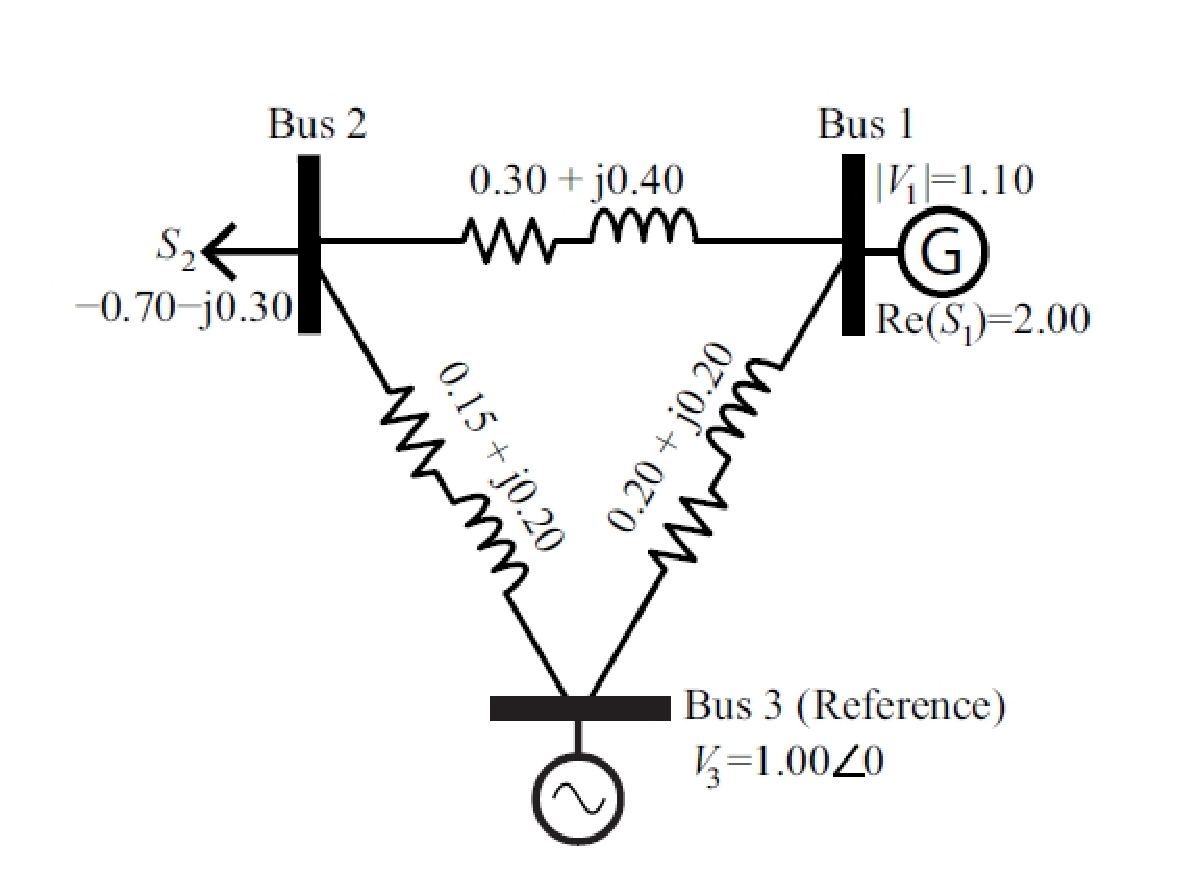
\includegraphics[width=9cm]{three_bus_system.eps}
% figure caption is below the figure
\caption{Three-bus system}
\label{fig:3bus}       % Give a unique label
\end{figure}
Power flow equations take the form
\begin{align*}
P_1 & = x^T \left(
              \begin{array}{cccc}
                3.7 & -0.6 & 0 & -0.8 \\
                -0.6 & 0 & 0.8 & 0 \\
                0 & 0.8 & 3.7 & -0.6 \\
                -0.8 & 0 & -0.6 & 0 \\
              \end{array}
            \right) x + \\
            & + 2 (( -1.25,    0,    1.25,    0)^T, x),\\
V_1 & = x_1^2 + x_3^2, \\
P_2 & =x^T \left(
              \begin{array}{cccc}
              0 & -0.6 & 0 & 0.8 \\
                -0.6 & 3.6 & -0.8 & 0 \\
                0 & -0.8 & 0 & -0.6 \\
                0.8 & 0 & -0.6 & 3.6 \\
              \end{array}
            \right) x + \\
            & + 2 (( 0, -1.2,    0,    1.6)^T, x),\\
Q_2 & =x^T \left(
              \begin{array}{cccc}
            0 & -0.8 & 0 & -0.6 \\
                -0.8 & 4.8 & 0.6 & 0 \\
                0 & 0.6 & 0 & -0.8 \\
                -0.6 & 0 & -0.8 & 4.8 \\
              \end{array}
            \right) x + \\ & + 2 (( 0, -1.6,    0,    -1.2)^T, x).
\end{align*}
We remind that  $x = (\text{Re} V_1,~ \text{Re} V_2,~ \text{Im} V_1,~ \text{Im} V_2)^T$ and $V_3 = 1$ for slack bus. Starting at the given operation regime $P_1 = 2$, $V_1^2 = 1.21$, $P_2 = -0.7$, $Q_2 = -0.3$ we obtain at least two vectors $c$ identifying nonconvexity but it requires more computational effort than in previous examples. Although our routine is capable to catch nonconvexity with probability one we are not sure that obtained vectors describe all the nonconvexities for this system.

The example may look artificial since the line resistances are as high as the reactances. We run our algorithm for the five times larger line reactances to model transmission grid and still discover
nonconvexity of the image.

{\it Remark} We do not propose any routine to solve power flow equation, and we do not pretend to
compete with any power flow solvers, neither DC equations nor iterative methods. Our method is focused on the certification and numerical description of nonconvexities of the image that is the reason for inexactness of convex relaxation for OPF.





% For one-column wide figures use
%
% For two-column wide figures use
%\begin{figure*}
% Use the relevant command to insert your figure file.
% For example, with the graphicx package use
%  \includegraphics[width=0.75\textwidth]{example.eps}
% figure caption is below the figure
%\caption{Please write your figure caption here}
%\label{fig:2}       % Give a unique label
%\end{figure*}
%


%%%%%%%%%%%%%%%%%%%%%%%%%%%%%%%%%%%%%%%%%%%%%%%%%%%%%%%%%%%%%%%%%%%%%%%%%%%%%%%
%
%  SECTION
%
%%%%%%%%%%%%%%%%%%%%%%%%%%%%%%%%%%%%%%%%%%%%%%%%%%%%%%%%%%%%%%%%%%%%%%%%%%%%%%%

\section{Conclusions}
\label{conclusion}

We investigate the image of the quadratic mapping. For many
applications convexity and ''hidden convexity'' plays crucial role
for effectiveness of the numerical procedures based on convex
relaxations.

We attack the problem of checking feasibility for a given $y^0$.
First, we formulate the sufficient condition for infeasibility. Then
we discover the particular structure of nonconvexity in terms of the
intersection of the image with supporting hyperplane. We claim that
nonconvexity can be characterized by the vector $c$ of the
supporting hyperplane when it satisfies certain conditions.
Straightforward sampling in the space of $c$ has no chances for
success but we provide numerical algorithm based on dual
representation of the boundary oracle. This algorithm discovers
nonconvexity with probability one. Finally, having discovered
nonconvexity we formulate additional cutting constraint that
guarantees convexity of $F \cup \{(c_{+}, f) \leq z\}$ and
feasibility of $y^0\in$conv($F$) and $(c_{+},y^0) \leq z$.


\section*{Acknowledgements}
The authors are thankful Prof. Janusz
Bialek who gave us opportunity working together. The collaboration
between Institute for Control Sciences RAS and Center for Energy
Systems of Skolkovo Institute of Science and Technology is
gratefully acknowledged.


\appendix
\section{Lemma for $m=2$, $x\in \mathbb{C}^n$}
\label{app a}
%This is app~\ref{app_a}

\begin{lemma}\label{lem:m2complex}
For $m=2$, $x\in \mathbb{C}^n$ the set $F$ is convex.
\end{lemma}
\begin{proof}
Introduce $z = (u, v)^T \in \mathbb{C}^{m+1}$, $v \in \mathbb{C}$
and three functions
\begin{align*}
g_i(z)& = u^*A_i u + v u^*b_i + v^* b_i^* u, \quad i = 1, 2,\\
g_3(z)& = (\text{Re } v)^2, \\
g(z) & = (g_1(z), g_2(z), g_3(z))^T.
\end{align*}

These functions are homogeneous quadratic forms, and the image $$G =
\{g(z) : \|z\| = 1, z \in \mathbb{C}^{m+1}\} \in\mathbb{R}^3$$ is
convex due to the theorem on numerical range \cite{HT}. Thus its
conic hull $Q = \{\lambda G, \lambda \geq 0\} \in \mathbb{R}^3$ is
also convex. But
\begin{align*}
Q & =\{\lambda g(z): \|z\| = 1, z\in \mathbb{C}^{m+1}, \lambda \geq
0\}
\\
& =\{g (\sqrt{\lambda} z): \|z\|=1, z\in \mathbb{C}^{m+1}, \lambda
\geq 0\}\\
& = \{g(z), z\in \mathbb{C}^{m+1}\}. \end{align*} Then its cross
section by the hyperplane $g_3 = 1$ is convex as well: $H =
\{(g_1(z),g_2(z))^T : g_3(z) = 1\}$ is convex. But $H$ coincides
with $F$. Indeed, $g_3 = 1$ implies either $\text{Re } v = 1$ and
then $g_i(z) = f_i(u)$, $i = 1,2$ or $\text{Re } v = -1$ and then
$g_i(z) = f_i(-u)$, $i = 1, 2$.
\end{proof}

% BibTeX users please use one of
%\bibliographystyle{spbasic}      % basic style, author-year citations
%\bibliographystyle{spmpsci}      % mathematics and physical sciences
%\bibliographystyle{spphys}       % APS-like style for physics
%\bibliography{bibenergy}   % name your BibTeX data base


\begin{thebibliography}{99}
%
% and use \bibitem to create references. Consult the Instructions
% for authors for reference list style.
%
%\bibitem{RefJ}
% Format for Journal Reference
%Author, Article title, Journal, Volume, page numbers (year)
% Format for books
%\bibitem{RefB}
%Author, Book title, page numbers. Publisher, place (year)
% etc

\bibitem{Barvinok95} A. Barvinok, Problems of distance geometry and convex
properties of quadratic maps {\it Discrete \& Computational
Geometry} 13(1), 189--202, (1995).

\bibitem{Ramana_NPhard94} M. Ramana and A. J. Goldman, Quadratic maps with convex
images. Rutgers University. Rutgers Center for Operations Research
[RUTCOR], 1994.

\bibitem{HT} Y.H. Au-Yeung and N.K.Tsing, An extension of the
Hausdorff�Toeplitz theorem on the numerical range, Proc. of the
Amer. Math. Soc. 89, 215-�219, (1983).


\bibitem{Low} S. Low, Convex Relaxation of Optimal Power Flow Part I: Formulations and Equivalence {\it
    IEEE Trans. on control of network systems}, 1(1), 15--27, (2014), Part II: Exactness, 1(2): 177--189,
    (2014).

\bibitem{Lowlect} S. Low, Mathematical Methods for Internet Congestion Control and Power System
    Analysis,
    Lecture Notes (in press).

\bibitem{LavaeiLow}
J. Lavaei and S. Low, Zero Duality Gap in Optimal Power Flow Problem
{\it IEEE Transactions on Power Systems}, 27(1), 92--107, (2012).

\bibitem{survey} S. Frank, I. Stepanovice and S. Rebennack, Optimal Power Flow: A Bibliographic Survey,
    Energy Systems, 2012, 221--289, (2012).


\bibitem{BTT} A. Ben-Tal and M. Teboulle, Hidden convexity in some nonconvex quadratically constrained
    quadratic programming, {\it Mathematical Programming}, 72(1), 51--63, (1996).

\bibitem{HUT} J.-B. Hiriart-Urruty, M. Torki, Permanently going back and forth between the ``quadratic
    world'' and the ``convexity world'' in optimization, {\it Appl. Math. and Optim.}, 45, 169--184, (2002).

\bibitem{LuoIEEE} Z.-Q. Luo, W.-K. Ma, A.M.-C. So, Y. Ye, S. Zhang, Semidefinite relaxation of quadratic
    optimization
    problems,
    {\it IEEE Sig. Proc. Magazine}, 27(3), (2010)

\bibitem{Zhang} S. Zhang, Quadratic optimization and semidefinite relaxation, {\it Mathematical
    Programming}, 87, 453�-465, (2000).

\bibitem{Dines} L.L. Dines, On the mapping of quadratic forms {\it Bull. Amer. Math. Soc.}, 47, 494--498,
    (1941).

\bibitem{Calabi} E. Calabi, Linear Systems of Real Quadratic Forms, {\it Proc. Amer. Math. Soc.}, 84(3),
    331--334, (1982).

\bibitem{polyak98} B.T. Polyak, Convexity of quadratic transformations and its use in control and
    optimization {\it Journal of Optimization Theory and Applications}, 99, 553--583, (1998).


\bibitem{Fradkov} A. L. Fradkov, Duality Theorems for Certain Nonconvex Extremum Problems, {\it
    Siberian Mathematical Journal}, 14, 247--264, (1973).

\bibitem{KK} S. Kim, M. Kojima, Exact Solutions of Some Nonconvex Quadratic Optimization Problems via
    SDP and SOCP Relaxations, {\it Computational Optimization and Applications}, 26, 143�-154, (2003).

\bibitem{Brickman}
L. Brickman, On the field of values of a matrix {\it Proc. Amer.
Math. Soc.}, 12, 61--66, (1961).

\bibitem{polyak01} B.T. Polyak, Convexity of nonlinear image of a small ball with applications to
    optimization {\it Set-Valued Analysis}, 9(1/2), 159--168, (2001).


\bibitem{Shor} N.Z.Shor, Quadratic Optimization Problems, {\it Soviet J. of Computer and Syst. Sci.},
    25(6), 1--11, (1987).

\bibitem{Beck} A. Beck, On the convexity of a class of quadratic mappings and
its application to the problem of finding the smallest ball
enclosing a given intersection of balls, {\it J. of Global Opt.},
39(1),  113--126, (2007).

\bibitem{Boyd} S. Boyd, L. El Ghaoui, E. Feron, and V. Balakrishnan, Linear Matrix Inequalities in System
    and Control Theory, Volume 15 of Studies in Applied Mathematics Society for Industrial and Applied
    Mathematics (SIAM), (1994).


%\bibitem{Gutkin} E. Gutkin, E. A. Jonckheere, M. Karow, Convexity of
%the joint numerical range: topological and differential geometric
%viewpoints, {\it Linear Algebra Appl.},  376, 143-171, (2004)


\bibitem{Ortega15} N. Barabanov, R. Ortega, R. Grino and B. Polyak, On existence and stability of
    equilibria of linear time-invariant systems with constant power loads {\it IEEE Transactions on Circuits
    and Systems I} (accepted).

\bibitem{DymTur_MITconf} A. Dymarsky and K. Turitsyn, Convex partitioning of the power flow feasibility
    region, (in press).

\bibitem{Suetin15}
S. Baghsorkhi and S. Suetin, Embedding AC Power Flow with Voltage
Control in the Complex Plane : The Case of Analytic Continuation via
Pade Approximants, {\it  arXiv:1504.03249}.

\bibitem{Dymarsky_SmallBall}
A. Dymarsky, Convexity of a Small Ball Under Quadratic Map, {\it
arXiv:1410.1553}.

\bibitem{Dymarsky_cuttingArX}
A. Dymarsky, On the Convexity of Image of a Multidimensional
Quadratic Map, {\it arXiv:1410.2254}.


\end{thebibliography}


\end{document}
% end of file template.tex
